\chapter{Perambatan Cahaya Menurut Garis Lurus}\label{ch:g6:light-propagation}

``\omterm{def:g1:light-and-shadows:source}{Cahaya} merambat menurut garis lurus'' sudah melayanimu selama dua
tahun --- menerangi \omterm{def:g1:light-and-shadows:shadow}{bayang-bayang}, membidikkan \omterm{def:g5:mirrors-reflection:reflection}{cermin}, menyejajarkan
tiga kartu dan sebatang lilin. Tahun ini hukum lama itu mendapat nama
resminya, aturan menggambarnya, dan akibatnya yang paling ajaib:
sebuah kamera tanpa lensa, tanpa kaca, tanpa bagian yang bergerak ---
hanya sebuah lubang.

\section{Hukumnya, dinyatakan dengan benar}

\begin{proposition}[Perambatan cahaya menurut garis lurus]\label{prop:g6:light-propagation:law}
Di \omterm{def:g2:air-around-us:air}{udara} yang bening --- dan di dalam bahan bening yang tercampur rata
seperti air yang tenang atau kaca --- \omterm{def:g1:light-and-shadows:source}{cahaya} merambat menurut garis
lurus. Inilah hukum \emph{perambatan lurus}\index{perambatan lurus}:
\emph{lurus} sekadar berarti ``menurut garis lurus'', dan
\emph{perambatan} menyebut perjalanan \omterm{def:g1:light-and-shadows:source}{cahaya} dari tempat ke tempat.
\end{proposition}

\begin{definition}[Sinar dan berkas]\label{def:g6:light-propagation:ray}
Sebuah \emph{sinar cahaya}\index{sinar cahaya} adalah gambar milik
fisikawan untuk satu helai \omterm{def:g1:light-and-shadows:source}{cahaya}: garis lurus dengan anak panah untuk
arah perjalanannya. Lampu yang sungguhan mencurahkan helai yang tak
terhitung banyaknya sekaligus: seikat sinar disebut
\emph{berkas}\index{berkas}. Tiga bentuk berkas sudah meliput
praktiknya: \emph{menyebar} (sinar yang memencar dari sebuah titik ---
lampu kecil mana pun), \emph{sejajar} (sinar yang berdampingan, tidak
bertemu maupun berpisah --- \omterm{def:g1:light-and-shadows:source}{cahaya} matahari, karena sudah menempuh
jarak yang begitu jauh), dan \emph{mengumpul} (sinar yang merapat
menuju sebuah titik --- \omterm{def:g1:light-and-shadows:source}{cahaya} yang dikumpulkan alat yang akan kamu
temui dua tahun lagi).
\end{definition}

\begin{omfigure}
\begin{tikzpicture}[scale=0.8]
  \fill[omThm] (0.5,1.3) circle (0.14);
  \foreach \a in {-28,-14,0,14,28} {
    \draw[-Stealth, omThm, thick] (0.6,1.3) -- ++(\a:2.6);
  }
  \node[below, font=\small] at (1.8,-0.1) {menyebar};
  \foreach \y in {0.5,1.0,1.5,2.0} {
    \draw[-Stealth, omThm, thick] (4.6,\y) -- (7.4,\y);
  }
  \node[below, font=\small] at (6.0,-0.1) {sejajar};
  \foreach \a in {152,166,180,194,208} {
    \draw[-Stealth, omThm, thick] (11.4,1.3) ++(\a:2.6)
      -- ++({\a-180}:2.35);
  }
  \fill[omExo] (11.4,1.3) circle (0.1);
  \node[below, font=\small] at (9.8,-0.1) {mengumpul};
\end{tikzpicture}

{\small Tiga \omterm{def:g6:light-propagation:ray}{berkas}: memencar dari sebuah lampu, berbaris sejajar dari
Matahari yang jauh, merapat menuju sebuah titik.}
\end{omfigure}

\begin{omfigure}
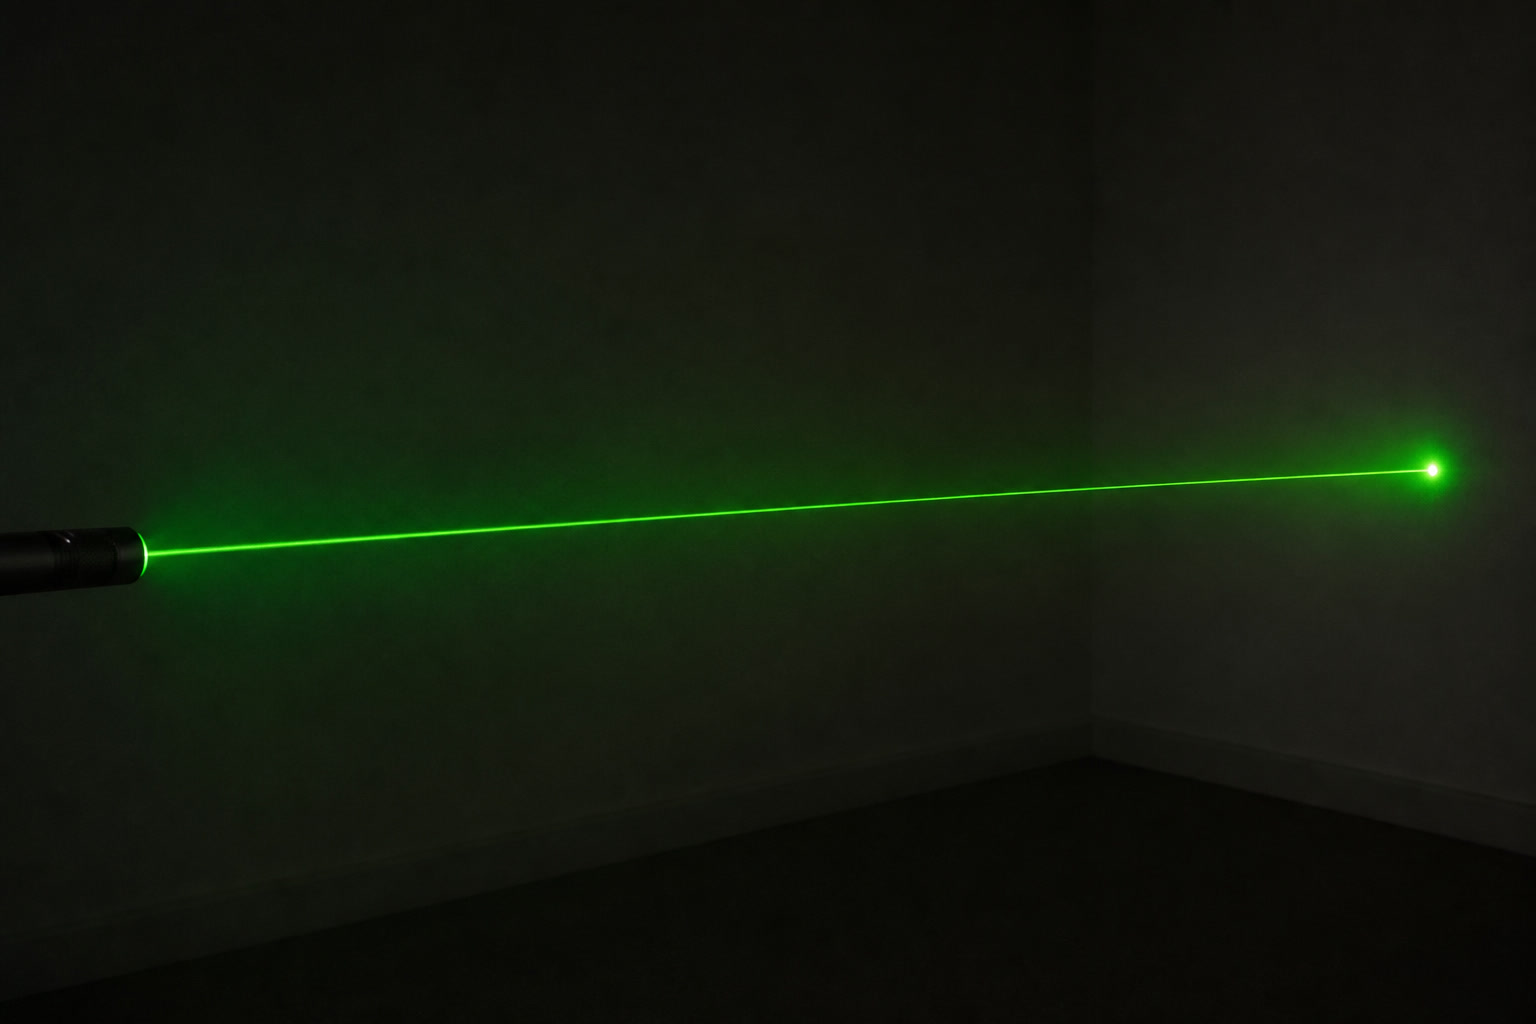
\includegraphics[width=0.55\linewidth]{images/book1/ai/g6-light-laser-fog.jpg}

{\small \omterm{def:g6:light-propagation:ray}{Berkas} laser yang ditampakkan oleh kabut: satu garis lurus sempurna dari sumbernya sampai ke dinding.}
\end{omfigure}

\begin{example}[Hukumnya bekerja, di mana-mana]\label{ex:g6:light-propagation:sightings}
Tukang bangunan membidik menyusuri tepi sebuah papan lurus untuk
menilainya --- mata, tepi, dan ujung jauhnya harus sebaris, dan
kelurusan cahayalah sumpah sang hakim. Juru ukur menancapkan tiang
sebaris dengan mata; pemanah dan juru foto ``menyejajarkan bidikan'';
dan percobaan tiga kartu dua tahun lalu kini punya nama resmi: sebuah
uji \omterm{prop:g6:light-propagation:law}{perambatan lurus}. Setiap satunya menukar garis lurus \omterm{def:g1:light-and-shadows:source}{cahaya} dengan
garis lurus benda.
\end{example}

\section{Bayang-bayang, dikonstruksi}

\begin{method}[Mengonstruksi bayang-bayang dengan penggaris]\label{met:g6:light-propagation:shadow}
Untuk lampu kecil $S$, sebuah bola, dan layar di belakangnya:
\begin{enumerate}
  \item gambarlah sinar dari $S$ yang tepat menyerempet tepi atas
        bolanya, lalu panjangkan lurus sampai ke layarnya;
  \item begitu pula sinar yang menyerempet tepi bawahnya (dan, dalam
        tiga dimensi, di seluruh kelilingnya);
  \item di antara kedua titik serempetan pada layarnya terletak
        \emph{bayang-bayang}\index{bayang-bayang}: daerah yang tidak
        dapat dicapai sinar lurus mana pun dari $S$;
  \item ruang di antara bola dan layar yang dibatasi sinar serempetan
        itu adalah \emph{kerucut \omterm{def:g1:light-and-shadows:shadow}{bayang-bayang}}: mata yang berada di
        dalamnya tidak dapat melihat lampunya.
\end{enumerate}
Tidak ada tebak-tebakan di mana pun: dua garis penggaris menetapkan
ukuran dan letak \omterm{def:g1:light-and-shadows:shadow}{bayang-bayangnya} dengan persis.
\end{method}

\begin{omfigure}
\begin{tikzpicture}[scale=0.8]
  \fill[omThm] (0.5,1.9) circle (0.15);
  \node[below, font=\small] at (0.5,1.6) {lampu};
  \draw[thick, fill=omDef, fill opacity=0.3] (4.4,1.9) circle (0.7);
  \draw[very thick] (9.8,-0.6) -- (9.8,4.4);
  \draw[omThm, thick] (0.62,1.99) -- (9.8,3.55);
  \draw[omThm, thick] (0.62,1.81) -- (9.8,0.25);
  \draw[line width=3.5pt, omExo] (9.8,0.25) -- (9.8,3.55);
  \node[right, font=\small] at (9.95,1.9) {bayang-bayang};
  \node[right, font=\small] at (9.95,4.1) {layar};
  \node[font=\small, omExo] at (7.2,1.9) {kerucut bayang-bayang};
\end{tikzpicture}

{\small \omterm{def:g1:light-and-shadows:shadow}{Bayang-bayang}, dibangun dengan dua sinar serempetan: segala
yang berada di antara kedua titik pendaratannya berada di luar
jangkauan \omterm{def:g1:light-and-shadows:source}{cahaya} yang lurus.}
\end{omfigure}

\begin{example}[Lebih besar, lebih kecil, lebih tajam]\label{ex:g6:light-propagation:sizes}
Konstruksinya meramalkan apa yang dahulu ditemukan permainan
mainan-dan-senter pada tahun pertamamu: geserlah bolanya ke arah lampu
dan sinar serempetannya mengipas lebih lebar --- \omterm{def:g1:light-and-shadows:shadow}{bayang-bayang}
raksasa; geserlah ke arah layar dan keduanya mendarat lebih rapat ---
\omterm{def:g1:light-and-shadows:shadow}{bayang-bayang} seukuran aslinya. Dan ramalannya persis: dengan bolanya
di tengah antara lampu dan layar, sinar serempetannya merentang dua
kali lebar bolanya --- \omterm{def:g1:light-and-shadows:shadow}{bayang-bayang} yang tepat dua kali ukuran
bolanya. Kesebandingan, digambar dengan \omterm{def:g1:light-and-shadows:source}{cahaya}.
\end{example}

\section{Kamera tanpa lensa}

\begin{method}[Membuat kamera lubang jarum]\label{met:g6:light-propagation:pinhole}
\begin{enumerate}
  \item ambillah sebuah kotak (kotak sepatu sudah cukup); di tengah
        salah satu ujungnya, buatlah lubang bersih sebesar jarum;
  \item gantilah ujung yang berseberangan dengan kertas jiplak ---
        inilah layarnya;
  \item selubungi kepalamu dan ujung berlayar itu dengan kain, lalu
        arahkan lubangnya ke pemandangan yang terang --- jendela,
        jalan yang terkena matahari;
  \item pandanglah kertas jiplaknya: pemandangannya muncul,
        berwarna, bergerak selagi pemandangannya bergerak ---
        \emph{terbalik}.
\end{enumerate}
\end{method}

\begin{proposition}[Mengapa bayangannya terbalik]\label{prop:g6:light-propagation:inverted}
\omterm{prop:g6:light-propagation:law}{Perambatan lurus} membangun gambarnya dan membalikkannya dalam satu
tarikan yang sama. Dari puncak pemandangannya, sinar berjalan lurus
menembus lubangnya --- dan garis lurus dari titik yang tinggi lewat
lubang yang rendah pasti melanjutkan perjalanannya \emph{ke bawah}:
puncaknya mendarat di dasar layarnya. Dari dasar pemandangannya, ia
naik lewat lubangnya sampai ke puncak layarnya. Setiap titik
pemandangannya mengirim helainya lewat satu gerbang kecil itu,
helai-helainya bersilangan di gerbangnya, dan gambarnya tersusun
terbalik --- atas menjadi bawah, kiri menjadi kanan.
\end{proposition}

\begin{omfigure}
\begin{tikzpicture}[scale=0.8]
  \draw[-Stealth, very thick, omDef] (0.7,0.6) -- (0.7,3.2);
  \node[left, font=\small] at (0.55,1.9) {pemandangannya};
  \draw[thick] (5.6,-0.2) -- (5.6,1.55) (5.6,2.05) -- (5.6,3.8);
  \node[above, font=\small] at (5.6,3.85) {dinding berlubang jarum};
  \draw[omThm, thick] (0.7,3.2) -- (5.6,1.8) -- (10.4,0.42);
  \draw[omThm, thick] (0.7,0.6) -- (5.6,1.8) -- (10.4,2.85);
  \draw[very thick] (10.4,-0.2) -- (10.4,3.8);
  \draw[-Stealth, very thick, omDef] (10.4,2.85) -- (10.4,0.42);
  \node[right, font=\small] at (10.55,1.6)
    {bayangannya: terbalik};
\end{tikzpicture}

{\small Kamera lubang jarum: setiap helai \omterm{def:g1:light-and-shadows:source}{cahaya} berjalan lurus
menembus gerbang kecilnya, helai-helainya bersilangan, dan
pemandangannya mendarat terbalik di layarnya.}
\end{omfigure}

\begin{remark}[Kotak yang tua dan terhormat]\label{rem:g6:light-propagation:history}
Ruang berlubang jarum --- \emph{camera obscura}, ``kamar gelap'' ---
berabad-abad lebih tua daripada fotografi: para astronom mengamati
gerhana dengan aman di layarnya, dan para pelukis menjiplak
\omterm{prop:g5:mirrors-reflection:image}{bayangannya} untuk mendapatkan perspektif yang benar. Setiap kamera
zaman sekarang, dan matamu sendiri, mempertahankan tata bangunannya:
gerbang kecil bagi \omterm{def:g1:light-and-shadows:source}{cahayanya}, layar bagi \omterm{prop:g5:mirrors-reflection:image}{bayangannya} --- dan ya,
\omterm{prop:g5:mirrors-reflection:image}{bayangan} di bagian belakang matamu pun berdiri terbalik; otakmu dengan
sopan membaliknya. Satu hukum garis lurus, yang diikuti dengan sabar,
menjelaskan kamera keluarga dan separuh sejarah pembuatan gambar.
\end{remark}

\section{Latihan}

\begin{exercise}[$\star$]\label{exo:g6:light-propagation:1}
Katakan hukum \omterm{prop:g6:light-propagation:law}{perambatan lurus} dengan kata-katamu sendiri, lalu
uraikan kedua kata panjangnya.
\end{exercise}

\begin{exercise}[$\star$]\label{exo:g6:light-propagation:2}
Sebutkan ketiga bentuk \omterm{def:g6:light-propagation:ray}{berkas}, masing-masing dengan satu sumber atau
keadaan yang nyata. Dalam bentuk mana \omterm{def:g1:light-and-shadows:source}{cahaya} matahari tiba, dan
mengapa?
\end{exercise}

\begin{exercise}[$\star$]\label{exo:g6:light-propagation:3}
Seorang tukang bangunan membidik menyusuri tepi sebuah rak untuk
memeriksa kelurusannya. Apa yang berperan sebagai penggaris pada uji
ini? Hukum mana yang dipercayainya?
\end{exercise}

\begin{exercise}[$\star$]\label{exo:g6:light-propagation:4}
Pada konstruksi \omterm{def:g1:light-and-shadows:shadow}{bayang-bayang}, apa yang menetapkan tepi
\omterm{def:g1:light-and-shadows:shadow}{bayang-bayangnya} pada layar? Apa yang berlaku bagi mata yang
ditempatkan di dalam kerucut \omterm{def:g1:light-and-shadows:shadow}{bayang-bayangnya}?
\end{exercise}

\begin{exercise}[$\star$]\label{exo:g6:light-propagation:5}
Dengan \cref{ex:g6:light-propagation:sizes}: bolanya berada di tengah
antara lampu dan layar. Bolanya selebar \qty{6}{cm} --- selebar apa
\omterm{def:g1:light-and-shadows:shadow}{bayang-bayangnya}? Dan kalau bolanya bergerak dekat ke layar?
\end{exercise}

\begin{exercise}[$\star$]\label{exo:g6:light-propagation:6}
Pada kamera lubang jarum, di mana \omterm{def:g1:light-and-shadows:source}{cahaya} dari puncak pemandangannya
mendarat pada layar? Telusuri alasannya dalam satu kalimat.
\end{exercise}

\begin{exercise}[$\star$]\label{exo:g6:light-propagation:7}
Seorang teman melambaikan tangan kanannya di depan kamera lubang
jarummu. Pada layarnya, sisi mana yang melambai, dan menghadap ke arah
mana? (Hati-hati --- ada dua pembalikan.)
\end{exercise}

\begin{exercise}[$\star$]\label{exo:g6:light-propagation:8}
Sebutkan dua pemakai camera obscura, baik pada masa lalu maupun masa
kini, dan pekerjaan yang dilakukannya bagi masing-masing.
\end{exercise}

\begin{exercise}[$\star\star$]\label{exo:g6:light-propagation:9}
Konstruksikan (sketsalah dengan penggaris): lampu di kiri, sebuah
penghalang berbentuk koin, layar di kanan --- lalu pindahkan
\emph{lampunya} menjadi dua kali lebih jauh dari koinnya, dengan layar
tetap. Apa yang terjadi pada ukuran \omterm{def:g1:light-and-shadows:shadow}{bayang-bayangnya}, menurut
gambarmu sendiri? Cocokkan dengan kipas sinar serempetannya.
\end{exercise}

\begin{exercise}[$\star\star$]\label{exo:g6:light-propagation:10}
Pada hari yang cerah, \omterm{def:g1:light-and-shadows:shadow}{bayang-bayang} pohon tampak tajam; di bawah
langit yang mendung, \omterm{def:g1:light-and-shadows:shadow}{bayang-bayang} hampir lenyap. Jelaskan kedua
langit itu dengan sinar dan sumber --- ``lampu'' macam apa selapis
awan kelabu yang utuh itu?
\end{exercise}

\begin{exercise}[$\star\star$]\label{exo:g6:light-propagation:11}
\omterm{prop:g5:mirrors-reflection:image}{Bayangan} kamera lubang jarum menjadi lebih terang ketika lubangnya
dilebarkan --- tetapi menjadi kabur. Jelaskan kedua akibatnya dengan
helai yang melewati gerbangnya: apa yang dibiarkan gerbang yang lebar
dilukiskan oleh tiap titik pemandangan pada layarnya?
\end{exercise}

\begin{exercise}[$\star\star\star$]\label{exo:g6:light-propagation:12}
Di bawah pohon yang rimbun ketika terjadi gerhana matahari sebagian,
tanahnya dipenuhi ratusan \omterm{ex:g2:moon-in-the-sky:shapes}{sabit} kecil. Susunlah penjelasannya dari bab
ini: apa sebenarnya celah di antara dedaunan itu, apa sebenarnya tiap
bercak terang pada hari biasa, dan mengapa bercaknya berubah menjadi
\omterm{ex:g2:moon-in-the-sky:shapes}{sabit} ketika Matahari berubah begitu? (Bab gerhana tahun depan akan
bangga kepadamu.)
\end{exercise}

\section{Soal: Panggung Bayang-bayang}

\begin{problem}[{Soal akhir pekan --- panggung bayang-bayang
keluarga; boneka yang diukur dengan kesebandingan, penutup berlubang
jarum; garis lurus cahaya yang menjalankan
pertunjukan}]\label{pb:g6:light-propagation:1}
Sehelai seprai sebagai layar, satu lampu kecil yang terang, boneka
karton: malam pembukaannya hari Sabtu, dan awak panggungnya bekerja
dengan penggaris.

\medskip\noindent\textbf{Bagian I --- Menyiapkan panggung.}
Lampunya berdiri \qty{4}{m} dari layarnya.
\begin{enumerate}
  \item Sebuah boneka yang ditempelkan pada layarnya melemparkan
        \omterm{def:g1:light-and-shadows:shadow}{bayang-bayang} tepat seukuran dirinya. Mengapa?
  \item Boneka naganya setinggi \qty{20}{cm}. Kalau dipegang di
        tengah --- \qty{2}{m} dari lampu dan dari layar --- setinggi
        apa \omterm{def:g1:light-and-shadows:shadow}{bayang-bayangnya}?
  \item Untuk babak penutup, naganya harus menjulang setinggi
        \qty{80}{cm}. Awaknya menggesernya ke arah lampu: pada jarak
        $1$ \omterm{def:g2:measuring-length:units}{meter} dari lampu, sinar serempetannya merentang empat
        kali ukuran bonekanya. Periksalah: cocokkah \qty{80}{cm}
        itu, dan pada pecahan berapa dari jarak lampu ke layar
        bonekanya berdiri?
  \item Mengapa lampu panggungnya harus kecil dan telanjang, bukan
        bola buram yang lebar? (Apa yang akan dilakukan bola itu
        terhadap tepi naganya yang tajam?)
\end{enumerate}

\medskip\noindent\textbf{Bagian II --- Seni panggung dengan sinar.}
\begin{enumerate}[resume]
  \item Boneka serigalanya harus membesar dengan mengancam selama
        babaknya tanpa lengan si dalang ikut muncul. Ke arah mana
        bonekanya digerakkan, dan apa yang terjadi pada tepi
        \omterm{def:g1:light-and-shadows:shadow}{bayang-bayangnya} selagi ia membesar? (Tepinya sedikit
        melembut --- terimalah lalu jelaskan dengan ukuran lampunya
        yang kecil tetapi bukan titik.)
  \item Dua boneka, yang dipegang pada jarak yang sama, tidak boleh
        saling menutupi \omterm{def:g1:light-and-shadows:shadow}{bayang-bayangnya}. Apa yang harus berlaku
        bagi garis lurus dari lampunya lewat tiap boneka?
  \item Sebuah tangan menyelinap di antara lampu dan naganya pada
        sepertiga jalan dari lampunya. \omterm{def:g1:light-and-shadows:shadow}{Bayang-bayang} siapa yang
        tampak lebih besar pada layarnya, tangan atau naga, dan
        mengapa?
  \item Sang penjahat harus lenyap seketika. Dengan sinar di tangan,
        berikan dua cara: satu dengan menggerakkan bonekanya, satu
        dengan memakai penghalang kedua yang lebih dekat.
\end{enumerate}

\medskip\noindent\textbf{Bagian III --- Penutup berlubang jarum.}
Untuk babak terakhir, awaknya mengubah panggungnya sendiri menjadi
camera obscura: lampu jalan di luar, lubang jarum pada daun jendela,
seprai layar melintang di dalam ruangan.
\begin{enumerate}[resume]
  \item Lampu jalannya tergantung tinggi di luar. Di mana
        \omterm{prop:g5:mirrors-reflection:image}{bayangannya} mendarat pada seprainya --- tinggi atau rendah?
        Mengapa?
  \item Seorang pesepeda yang pulang larut melintas dari kiri ke
        kanan. Ke arah mana \omterm{prop:g5:mirrors-reflection:image}{bayangan} pesepeda itu meluncur di
        seprainya?
  \item Penontonnya menginginkan gambar yang lebih terang, sehingga
        awaknya memperbesar lubang jarumnya menjadi bukaan sebesar
        koin. Apa jadinya pertunjukannya, dan mengapa?
  \item Baris penutup pada catatan acaranya: dalam satu kalimat,
        sebutkan satu hukum yang menjalankan seluruh malam itu ---
        kedua panggungnya, semua \omterm{def:g1:light-and-shadows:shadow}{bayang-bayangnya}, dan jalanan yang
        terbalik itu.
\end{enumerate}
\end{problem}
